\documentclass[11pt]{article}
\usepackage{amsmath, amssymb}
\usepackage{geometry}
\geometry{margin=1in}
\usepackage{fancyhdr}
\usepackage{lastpage}
\usepackage{parskip} % Better paragraph spacing
\usepackage{titlesec} % Better section formatting
\usepackage{graphicx}
\usepackage{float}
\usepackage[most]{tcolorbox}
\usepackage{lmodern}
\usepackage{caption}
\usepackage{hyperref}
\usepackage{listings}
\usepackage{xcolor}

\definecolor{codegreen}{rgb}{0,0.6,0}
\definecolor{codegray}{rgb}{0.5,0.5,0.5}
\definecolor{codepurple}{rgb}{0.58,0,0.82}
\definecolor{backcolour}{rgb}{0.95,0.95,0.92}

% Define code styling
\lstdefinestyle{mystyle}{
    backgroundcolor=\color{backcolour},
    commentstyle=\color{codegreen},
    keywordstyle=\color{magenta},
    numberstyle=\tiny\color{codegray},
    stringstyle=\color{codepurple},
    basicstyle=\ttfamily\footnotesize,
    breakatwhitespace=false,
    breaklines=true,
    captionpos=b,
    keepspaces=true,
    numbers=left,
    numbersep=5pt,
    showspaces=false,
    showstringspaces=false,
    showtabs=false,
    tabsize=2
}

\lstset{style=mystyle}

% Define commands for reusable content
\newcommand{\coursename}{CS-401 Applied Data Analysis}
\newcommand{\lecturenum}{12}
\newcommand{\lecturedate}{03/12/2025}
\newcommand{\professor}{Clément Pit-Clauded / Robert West}

\hypersetup{colorlinks=true,linkcolor=blue,urlcolor=blue}

% Configure section spacing
\titlespacing*{\section}{0pt}{2ex plus 1ex minus .2ex}{1.5ex plus .2ex}
\titlespacing*{\subsection}{0pt}{1.5ex plus 1ex minus .2ex}{1ex plus .2ex}
% Header / Footer
\pagestyle{fancy}
\fancyhf{}
\fancyhead[L]{\coursename}
\fancyhead[R]{Lecture \lecturenum}
\fancyfoot[L]{EPFL - Computer Science}
\fancyfoot[C]{Author: Jonathan Dutoit}
\fancyfoot[R]{Page \thepage\ of \pageref{LastPage}}

\begin{document}

\begin{center}
  {\large EPFL - Computer Science} \\[0.5em]
  {\Large \textbf{\coursename}} \\[0.5em]
  {\large Lecture \lecturenum\ --- \lecturedate} \\[0.5em]
  {\large Author: Jonathan Dutoit} \\[0.5em]
  {\large Professor: \professor} \\[0.5em]
\end{center}

\vspace{2cm}
\begin{center}
  {\LARGE \textbf{How to scale massive data}}
\end{center}

\vspace{1cm}

\section*{Warm up}

\begin{lstlisting}[language=Octave]
count = 0
for n in range(0, 10**9):
   if n.bit_count() == 5:
       count += 1
print(count)
\end{lstlisting}
\textbf{Question:} how long is this going to take? 1 billion operations, suppose \verb|n.bit_count()| is instantaneous (fast) and most CPU have optimization to that operation. Since modern CPUS run at 4-5GHz, one would expect it to take $< 1$ seconds. In the professor machine, it took surprisingly \textbf{51 seconds}. 

Also, this program is not doing anything interesting. If we had an interesting computation there, it would be even slower. Like cross-referencing large datasets. 

\textbf{Another question:} Does this course use \underline{Moodle}? The Moodle admins have a responsibility to log connections to track how the website is being used. Suppose it takes a couple of Gigabytes, this would already \textbf{be more than 1 billion...}

One year of Moodle logs:
\begin{lstlisting}[language=Octave]
14000 students
*  3-20 session per day
*    4-7 days per week
*     14 week per term
*      2 terms per year
*     3-5 pages per session
*    10-80 requets per page (!)
*  200-500 bytes per log entry
= 5500GB = 5.5TB
=     10 hours to read from a hard drive??
\end{lstlisting}

$\Rightarrow$ distribute, parallelize, stream

\textbf{So far in this class...}

\begin{itemize}
	\item We made one big assumption
		\begin{itemize}
			\item All data fits on a single machine
			\item Even more, all data fits into memory on a single machine (Pandas)
		\end{itemize}
	\item Realistic assumption for \textbf{prototyping}, but frequently not for production code
\end{itemize}
$\Rightarrow$ You need to be able to program the cloud

\section*{The big-data problem}

Data is growing fast than computation speed

\textcolor{green}{+ Growing data sources} 

\hspace{0.5cm}\textcolor{green}{(e.g., Web, mobile, sensors, ...)}

\textcolor{green}{+ Cheap hard-disk storage}

\vspace{0.5cm}

\textcolor{red}{- Slow read speeds $\Rightarrow$ Must distribute}

\textcolor{red}{- Stalling CPU speeds $\Rightarrow$ Must parallelize}

\textcolor{red}{- RAM bottlenecks $\Rightarrow$ Must stream}

\section*{Examples}
\textbf{Typical hard drive:} \$12 / TB (2024), 150 MB/s reads $\Rightarrow$ 2h / TB
\begin{itemize}
	\item All StackOverflow posts: 100 GB
	\item WSL (Swiss) rockslide measurements: 2 TB / day
	\item Worldwide stock-market data: 2.5 TB / day
	\item Github Arctic Code Vault: 21 TB
	\item Facebook daily logs, 2016: 60 TB / day
	\item Entire BrainMaps project: 140 TB
	\item Uber's analytics: PBs / day
	\item CERN's filtered experimental data: 1 PB / day
	\item Entire Wayback Machine archive: 99 PB
	\item CERN raw experimental data: 1 PB / second
\end{itemize}

\section*{But how much data should you get?}

Of course, "it depends", but for many applications the answer is: \textbf{As much as you can get}

Big data about people (text, Web, social media) tends to follow heavy-tailed distributors (e.g., power laws). Example: Web search. 

\textbf{Note}: \textbf{59\% of all Web search queries are unique}. 17\% of all queries are made only twice. 

\section*{The big-data problem}

A single machine can no longer store, let alone process, all the data. The solution is to \textbf{distribute} over a large cluster of machines. 

\textbf{Hardware for big data}
\begin{itemize}
	\item \textbf{Budget} (a.k.a. commodity) hardware. Not "gold-plated" (a.k.a. custom)
	\item Many low-end servers: \textbf{easy to add capacity}. \textbf{Cheaper} per CPU and per disk
	\item \textbf{Increased complexity in software:}
		\begin{itemize}
			\item Fault tolerance
			\item Virtualization (e.g., distributed file systems)
		\end{itemize}
\end{itemize}

\section*{Problems with cheap hardware}

\textbf{Failures}, e.g., (Google numbers)
\begin{itemize}
	\item 1-5\% hard drives/year
	\item 0.2\% DIMMs (dual in-line memory modules)/year
\end{itemize}

\textbf{Commodity network} (1-10 Gb/s) speeds vs. RAM
\begin{itemize}
	\item Much more latency (100-100,000x)
	\item Lower throughput (100-1,000x)
\end{itemize}

\textbf{Uneven performance}
\begin{itemize}
	\item Inconsistent hardware (e.g., old + new)
	\item Variable network latency
	\item External loads
\end{itemize}
% Quick centered image
\begin{figure}[H]
    \centering
    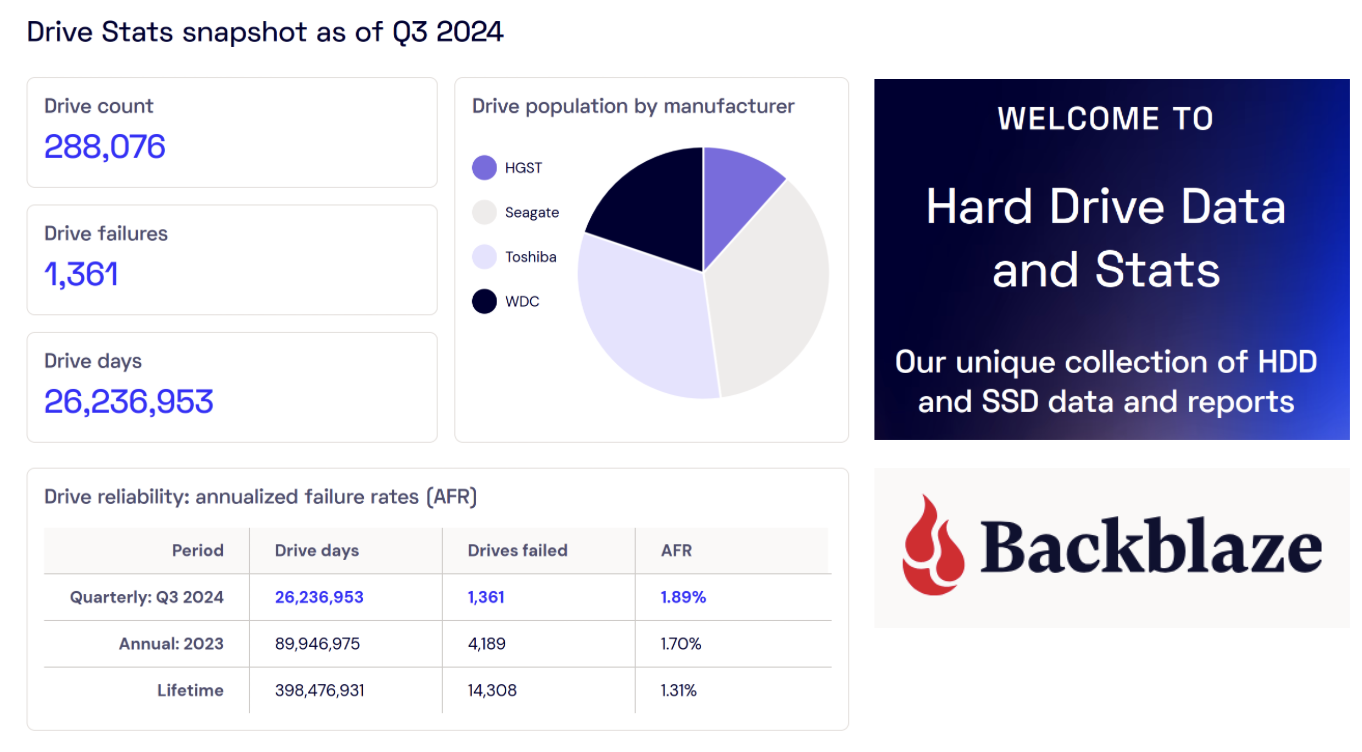
\includegraphics[width=0.8\textwidth]{backblaze}
    \label{fig:LABEL}
\end{figure}

\section*{What's hard about cluster computing?}

\textbf{1. How to split work across machines?}

\textbf{2. How to deal with failures?}

\vspace{0.5cm}

\begin{center}
  {\LARGE \textbf{Distributed aggregation}} \\
  Models of distributed computation
\end{center}
\vspace{0.5cm}


% Quick centered image
\begin{figure}[H]
    \centering
    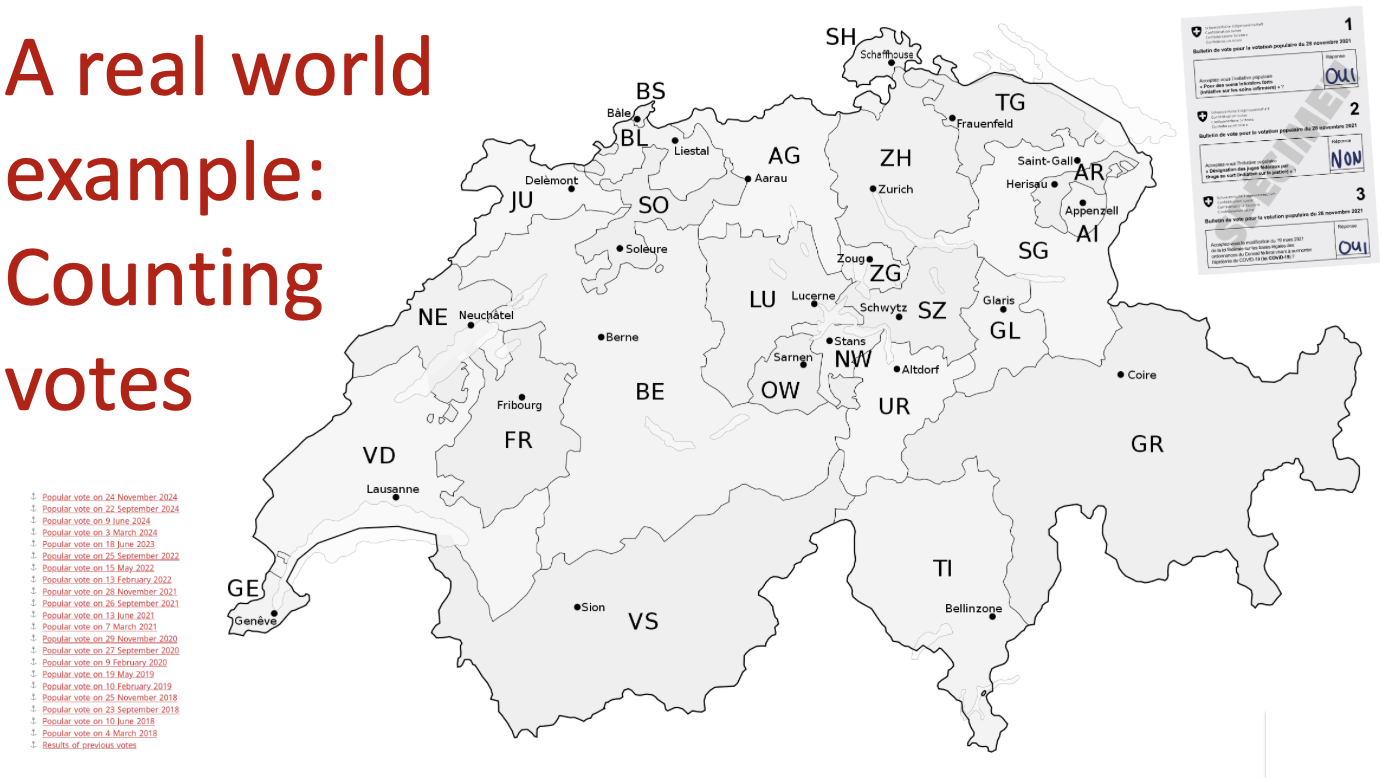
\includegraphics[width=0.8\textwidth]{voting}
    \label{fig:LABEL}
\end{figure}

\begin{itemize}
	\item First idea: \textbf{Truck full of ballots} going to Bern. Centralized collection, centralized counting. This is not ideal: shipping costs to transport all ballots. Also, voting participation is high in Switzerland: sequential count takes time! 
	\item Second ideal: \textbf{Train full of more ballots} going to Bern. \textbf{Distributed} collection, centralized counting. Transportation costs were highly reduced.
	\item Third idea: \textbf{One phone call} to Bern. Centralized collection, \textbf{distributed counting}.
	\item Fourth idea: \textbf{partial counts and use phone calls}! \textbf{Distributed} collection, \textbf{distributed} counting. 
\end{itemize}

\textbf{All distributed:}
% Quick centered image
\begin{figure}[H]
    \centering
    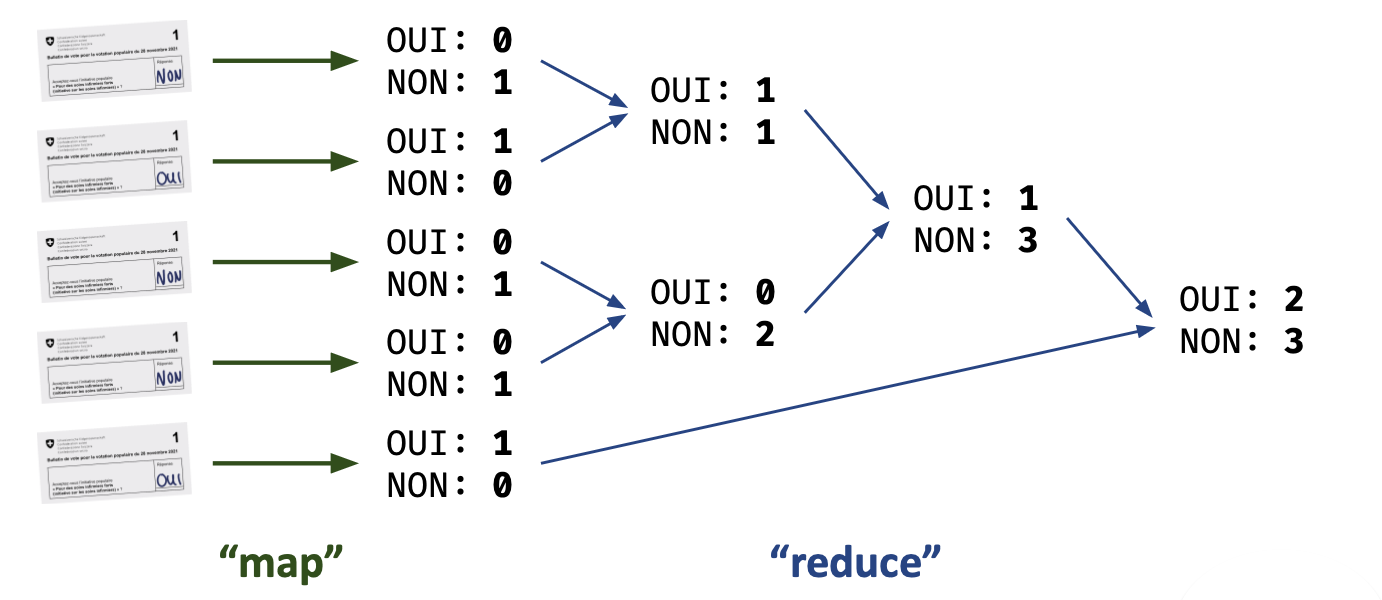
\includegraphics[width=0.6\textwidth]{distributed}
    \label{fig:LABEL}
\end{figure}

\vspace{0.5cm}

\begin{center}
  {\LARGE \textbf{MapReduce / Hadoop}} \\
  Models of distributed computation
\end{center}
\vspace{0.5cm}

How do you count the number of occurrences of each word in a document? We could do a \textcolor{red}{hashtable}! 

"I am Sam \\
\textcolor{red}{$[$}I\textcolor{red}{$]$} am Sam \\ 
Sam I am \\ 
Do you like \\
Green eggs and\\
ham?" 

\{I: \textcolor{red}{2}, am: 1, Sam: 1\}... What if the document is \textcolor{red}{REALLY} big?

\textbf{Divide and conquer!}
% Quick centered image
\begin{figure}[H]
    \centering
    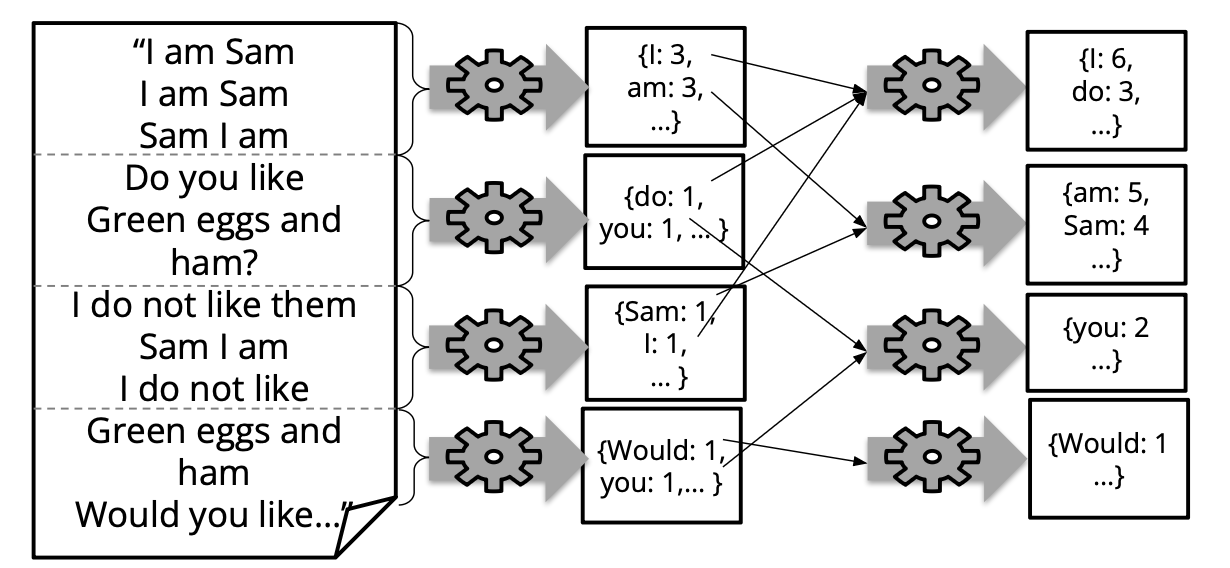
\includegraphics[width=0.6\textwidth]{sam-divide-and-conquer}
    \label{fig:LABEL}
\end{figure}

% Quick centered image
\begin{figure}[H]
    \centering
    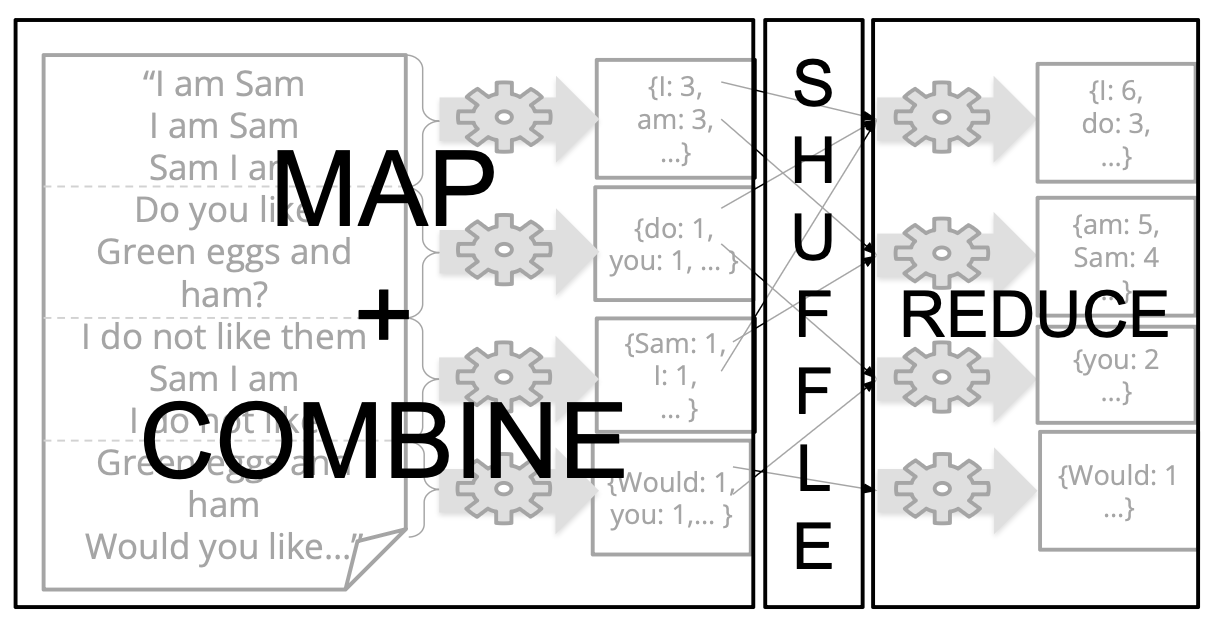
\includegraphics[width=0.5\textwidth]{sam-divide-and-conquer2}
    \label{fig:LABEL}
\end{figure}

1. How to divide work across machines?
\begin{itemize}
	\item Moving data may be very expensive
	\item Must consider network, data locality
\end{itemize}

2. How to deal with failures?
\begin{itemize}
	\item 1 server fails every 3 years $\Rightarrow$ 10K servers see $\sim$10 faults/day
	\item Even worse: stragglers (node not failed, but slow)
\end{itemize}

\textbf{Note}: checking whether a computer is going to finish its computation it's a well-known undecidable problem: \textbf{Halting problem}!
\newpage
\section*{Solution: MapReduce}

\begin{itemize}
	\item Smart systems engineers have done all the work for you (\textbf{hadoop}). 
		\begin{itemize}
			\item Task scheduling
			\item Virtualization of file system
			\item Fault tolerance (incl. data replication)
			\item Job monitoring
			\item etc.
		\end{itemize}
	\item "All" you need to do: implement Mapper and Reducer classes\\ 
		\textcolor{red}{Need to break more complex jobs into sequence of MapReduce jobs}
\end{itemize}

\textbf{\textcolor{red}{How to deal with failures?}} Just launch another task! 

\textbf{\textcolor{red}{How to deal with slow tasks?}} Just launch another task! 

\section*{Example Task}
% Quick centered image
\begin{figure}[H]
    \centering
    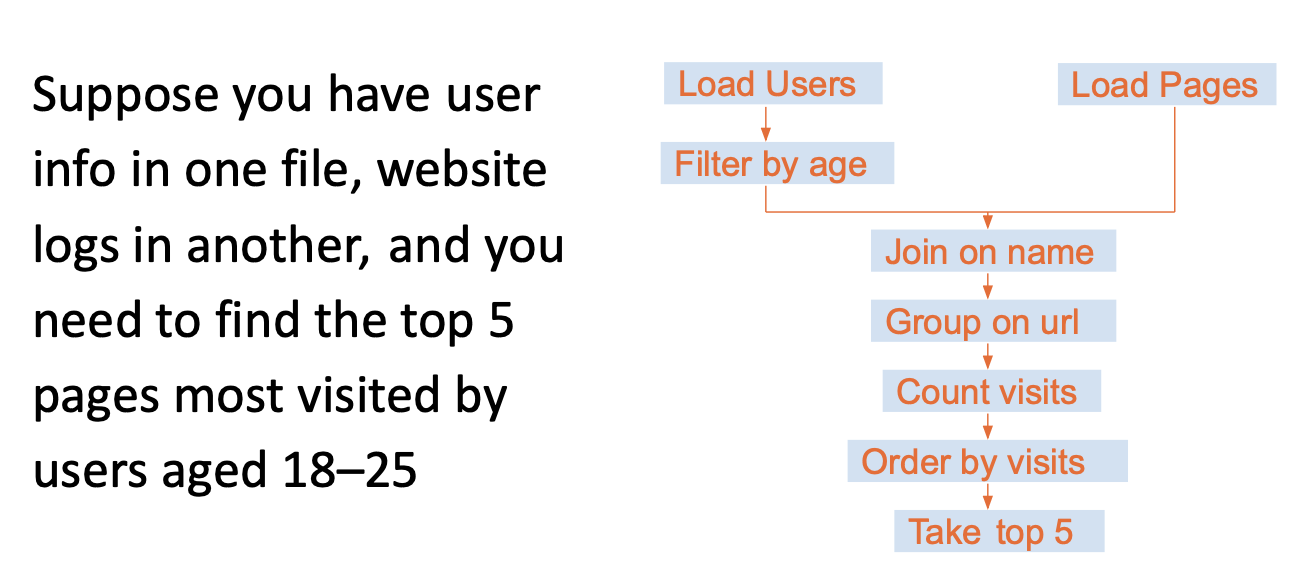
\includegraphics[width=0.6\textwidth]{example-task}
    \label{fig:LABEL}
\end{figure}

\section*{Example Task in MapReduce}
% Quick centered image
\begin{figure}[H]
    \centering
    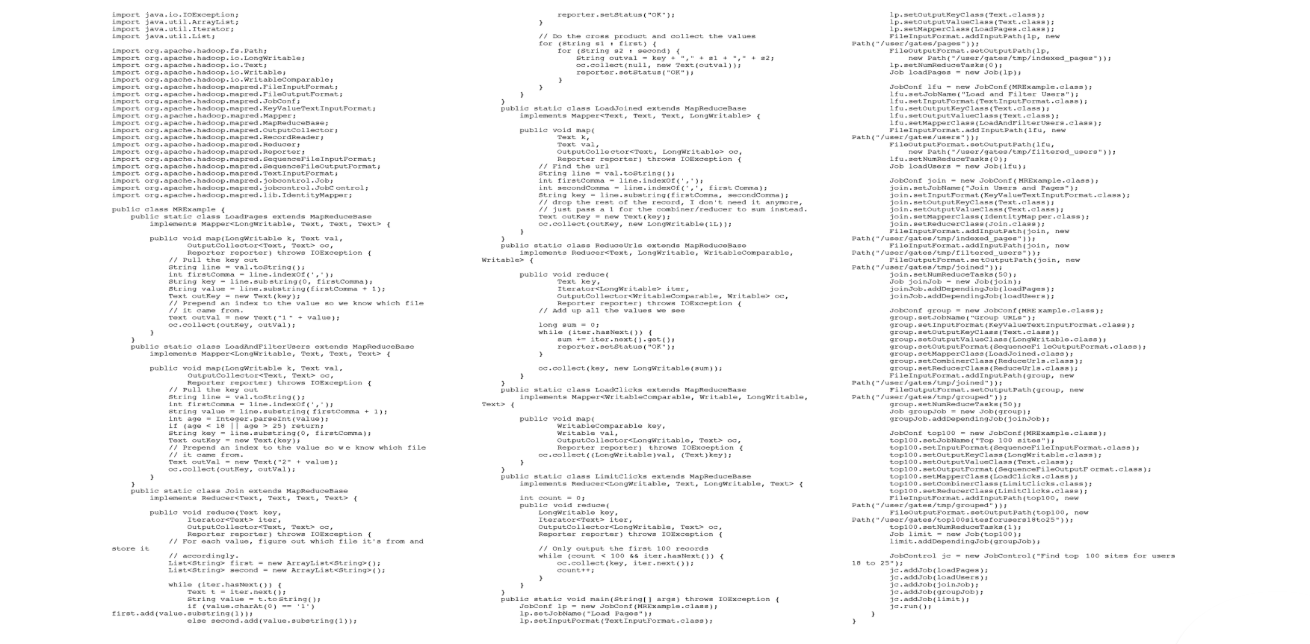
\includegraphics[width=0.8\textwidth]{example-task-mapreduce}
    \label{fig:LABEL}
\end{figure}

\section*{\textcolor{red}{Enter}: Spark}
\begin{itemize}
	\item A high-level fun(ctional) programming API
\end{itemize}
\begin{lstlisting}[language=Python]
print("I am a regular Python program, using pyspark")

users = (sc.textFile('users.tsv') # user <TAB> age
        	.map(lambda line: line.split('\t'))
        	.filter(lambda user_age: 18 <= int(user_age[l]) <= 25))

pages = (sc.textFile('pageviews/*.tsv')  # user <TAB> url
           .map(lambda line: line.split('\t')))

counts = (users.join(pages)
               .map(lambda user_age_url: (user_age_url[1][1], 1))
               .reduceByKey(lambda x, y: x + y)
               .takeOrdered(5))
\end{lstlisting}

This pretty closely mirrors the diagram and will faster than \verb|mapReduce|. Actually, for distributed cloud computing style programs, keeping programs as high-level as possible gives them higher optimization opportunities. 

\section*{Spark}

\begin{itemize}
	\item Implemented in \textbf{Scala} (go EPFL!)
	\item Additional APIs in 
		\begin{itemize}
			\item Python, Java, R
		\end{itemize}
	\item Many abstractions
		\begin{itemize}
			\item Core: RRDs
			\item Derived: dataframes, SQL, ML toolkit
		\end{itemize}
\end{itemize}

\vspace{0.5cm}

\begin{center}
  {\LARGE \textbf{RDDs: concepts}} \\
  Models of distributed computation
\end{center}
\vspace{0.5cm}

\section*{RDD: resilient distributed dataset}
\begin{itemize}
	\item To programmer: looks like one single collection (each elements represents a "row" of a dataset)
	\item Under the hood: oh boy...
		\begin{itemize}
			\item RDDs "live in the cloud": split over several machines, replicated, etc. 
			\item Can be processed in parallel
			\item Can be transformed to a single, real collection (if small...)
			\item Typically read from a distributed file system (HDFS)
			\item Can be written to a distributed file system
		\end{itemize}
\end{itemize}

\section*{Spark architecture}

% Quick centered image
\begin{figure}[H]
    \centering
    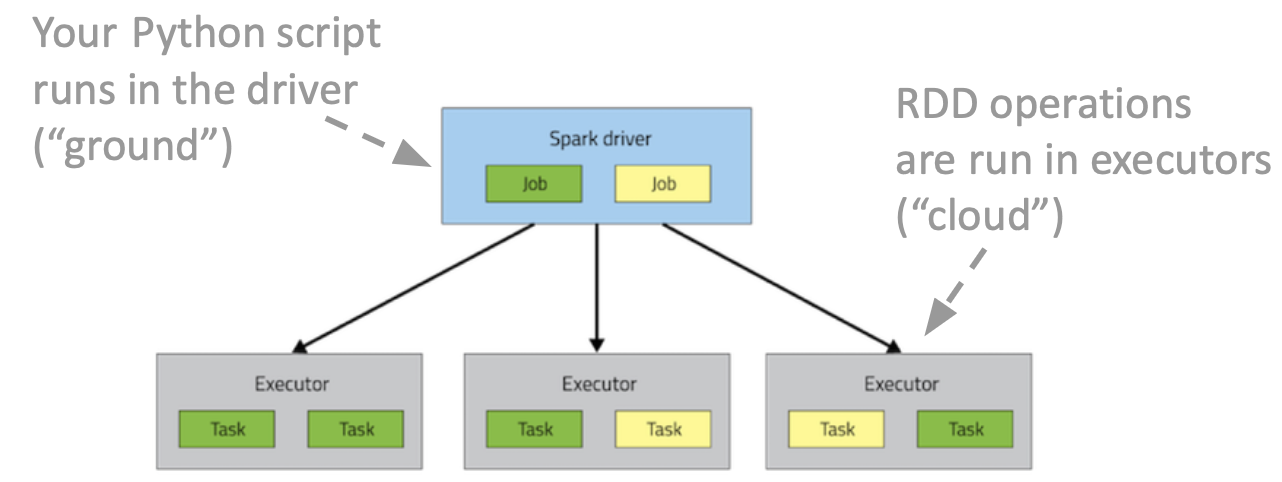
\includegraphics[width=0.6\textwidth]{spark-architecture}
    \label{fig:LABEL}
\end{figure}
\begin{itemize}
	\item One executor is essentially one machine with multiple CPUs 
	\item One task is the fact of processing one partition of data
	\item Each task is run by one CPU. So one executor can execute multiple tasks at the same time. 
\end{itemize}

\section*{RDD operations}
\begin{itemize}
	\item \textbf{"Transformations"}
		\begin{itemize}
			\item Input: RDD; output: another RDD
			\item Everything remains "in the cloud" 
			\item Example: for every entry in the input RDD, count chars 
				\begin{itemize}
					\item RDD: \{'I', 'am', 'you'\} $\Rightarrow$ RDD:\{1, 2, 3\}
				\end{itemize}
		\end{itemize}
	\item \textbf{"Actions"}
		\begin{itemize}
			\item Input: RDD; output: a value that is returned to the driver
			\item Result is transferred "from cloud to ground"
			\item Example: take a sample of entries from RDD and print it on the driver's shell; or store results to file (local or distributed) 
		\end{itemize}
\end{itemize}

\section*{Lazy execution}
\begin{itemize}
	\item \textbf{Transformations} (i.e., RDD $\Rightarrow$ RDD operations) are not executed until it's really necessary (a.k.a. "lazy execution")
	\item Execution of transformations triggered by \textbf{actions}
	\item Why?
		\begin{itemize}
			\item If you never look at the data, there's no point in manipulating it...
		\end{itemize}
\end{itemize}

\section*{Exercises}
Rewrite the following to be more efficient:
\begin{itemize}
	\item \verb|rdd.sort().first() == rdd.min()|
	\item \verb|rdd.map(f).map(g) == rdd.map(lambda x: g(f(x))|
\end{itemize}

Implement map and filter using only \verb|flatMap|

\begin{itemize}
	\item \verb|rdd.map(f) == rdd.flatMap(lambda x: [f(x)])|
	\item \verb|rdd.filter(f) == rdd.flatMap(lambda x: [x] if f(x) else [])|
\end{itemize}

\section*{RDD transformations}

\begin{itemize}
	\item \textbf{sample}\verb|(withReplacement?, fraction, seed)|: Sample a \textit{fraction} of the data, with or without replacement, using a given random number generator \textit{seed}
	\item \textbf{union}\verb|(otherDataset)|: New dataset that contains the union of the source and the argument.
	\item \textbf{intersection}\verb|(otherDataset)|:...
	\item \textbf{distinct}\verb|()|: New dataset that contains distinct elements of the source
	\item \textbf{groupByKey}(): When called on a dataset of (K, V) pairs, returns a dataset of \verb|(K, Iterable<V>)| pairs.
	\item \textbf{reduceByKey}\verb|(func)|: when called on dataset of (K, V) pairs, returns a dataset of (K, V) pairs where the values for each key are aggregated using the given reduce function \verb|func|, which must be of type (V, V) $=>$ V
	\item \textbf{reduce}\verb|(func)|: ?? (Needs associativity (unordered dataset) and commutativity (ordered dataset))
	\item \textbf{sortByKey}\verb|()|: When called on a dataset of (K, V) pairs, returns a dataset of (K, V) pairs sorted by keys
	\item \textbf{join\verb|(otherDataset)|}: When called on datasets of type (K, V) pairs and (K, W) pairs, returns a dataset of (K, (V, W)) pairs with all pairs of elements for each key (default is a \textbf{left-join})
	\item Analogous: \textbf{leftOuterJoin}, \textbf{rightOuterJoin}, \textbf{fullOuterJoin}

\end{itemize}

\section*{RDD actions}

\begin{itemize}
	\item \textbf{collect()}: Return all the elements of the dataset as an array at the driver program. This is usually useful after a filter or other operation that returns a sufficiently small subset of the data.
	\item \textbf{count}(): Return the number of elements in the dataset
	\item \textbf{reduce}\verb|(func)|: Compute a single value (\textbf{deterministic?})
	\item \textbf{take}\verb|(n)|: Return an array with the "first"\textit{n} elements of the dataset.
	\item \textbf{saveAsTextFile}\verb|(path)|: Save to local filesystem or HDFS
\end{itemize}

\section*{Broadcast variables}

\begin{minipage}{0.48\textwidth}
\begin{lstlisting}[language=Octave]
my_set = set(...)
rdd2 = rdd1.filter(lambda x: x in my_set)
\end{lstlisting}
This is a bad idea: \verb|my_set| needs to be shipped with every task (one task per data partition, so if \verb|rdd1| is spread over \textit{N} partitions, the above will require copying the same object \textit{N} times)
\end{minipage}
\hfill
\begin{minipage}{0.48\textwidth}
\begin{lstlisting}[language=Octave]
my_set = sc.broadcast(set(...))
rdd2 = rdd1.filter(lambda x: x in my_set.value)
\end{lstlisting}
This way, \verb|my_set| is copied to each executor only once and persists across all tasks (one per partition) on the same executor
\end{minipage}

\textbf{Note}: broadcast variables are \textbf{read-only}

\section*{Accumulators}

\begin{minipage}{0.48\textwidth}
\begin{lstlisting}[language=Octave]
def f(x): return x*2
rdd2 = rdd1.map(f)
\end{lstlisting}
How can we easily know how many rows there are in rdd1 (without running a costly reduce operation)?
\end{minipage}
\hfill
\begin{minipage}{0.48\textwidth}
Side effects via accumulators!
\begin{lstlisting}[language=Octave]
counter = sc.accumulator(0)
def f(x): counter.add(1); return x*2
rdd2 = rdd1.map(f)
\end{lstlisting}
\end{minipage}

\begin{itemize}
	\item Accumulators are \textbf{write-only} ("add-only") for executors
	\item Only driver can read the value: \textcolor{red}{counter.}\textcolor{blue}{value}
\end{itemize}

\section*{How does Spark run?}
\begin{lstlisting}[language=Octave]
print("I am a regular Python program, using pyspark")

users = (sc.textFile('users.tsv') # user <TAB> age
           .map(lambda line: line.split('\t'))
           .filter(lambda user_age: 18 <= int(user_age[1]) <= 25))

views = (sc.textFile('pageviews/*.tsv')  # user <TAB> url
           .map(lambda line: line.split('\t')))

counts = (users.join(views)
               .map(lambda user_age_url: (user_age_url[1][1], 1))
               .reduceByKey(lambda x, y: x + y)
               .takeOrdered(5))

\end{lstlisting}

\vspace{0.5cm}

\begin{center}
  {\LARGE \textbf{Dataframes and SQL}} \\
  Models of distributed computation
\end{center}
\vspace{0.5cm}

\section*{Spark DataFrames}
\begin{itemize}
	\item Bridging the gap between your experience with Pandas and the need for distributed computing
		\begin{itemize}
			\item RDD = collection of records
			\item DataFrame = table with rows and typed columns
		\end{itemize}
	\item Important to understand what RDDs are and what they offer but today most of the tasks can be accomplished with DataFrames
\end{itemize}

\section*{Spark DataFrames}
\begin{lstlisting}[language=Octave]
users = spark.read.csv("users.csv", header=True)
views = spark.read.csv("pageviews/*.csv", header=True)
counts = (
    users[users.age.between(18, 25)]
      .drop("age")
      .join(views, on="name")
      .groupby("url").count()
      .sort_values("name", ascending=True)
      .head(5)
).toPandas()
\end{lstlisting}

\section*{Spark SQL}
\begin{lstlisting}[language=Octave]
counts = spark.sql("""
  SELECT url, COUNT(*)
  FROM users 
  JOIN views ON users.name == views.name
  WHERE 18 <= age AND age <= 25
  GROUP BY url
""")

counts.toPandas()
\end{lstlisting}

\end{document}
